
\section{问题背景}

在乡村振兴与农业现代化融合发展的背景下,科学规划并高效利用有限的土地资源,对于保障区域粮食安全和促进乡村经济可持续发展具有重要意义。该问题不仅涉及资源优化配置的运筹学建模,还关联到生态经济学中的经济—生态系统耦合机制,以及区域发展经济学中的内生增长动力培育。农作物的生产与选择受地域、气候和土壤条件等自然因素制约,同时其经济效益又依赖于市场需求、成本与价格等动态变量。因此,为特定乡村制定能够兼顾经济产出最大化、生态系统稳定性和风险应对能力的长期种植策略,是智慧农业研究的关键问题之一。

本研究以华北某山区乡村为研究对象,该乡村拥有包括露天耕地和设施大棚在内的多类型土地资源,同时受到作物轮作、豆类种植比例以及田间管理便利性等多重约束条件的影响。这些现实因素构成了一个多维、多约束的决策环境。本研究通过系统的数学建模方法,构建贯穿2024年至2030年的最优种植方案,以期为资源高效利用和经济稳健增长提供数据驱动的决策参考框架。


\section{问题重述}

问题一:在所有经济与生产参数取基准值且保持不变的条件下,针对 2024–2030 年规划期,求解最优种植结构以最大化七年累计利润。分别在两种需求情景下求解:(i)产量超出预期的部分无法销售;(ii)超出部分以基准价格的 50\% 出售。

问题二:在问题一框架上引入参数不确定性。考虑预期销售量、单位面积产量、单位面积种植成本和销售价格在给定区间内的波动,设计一个在整个规划期内保持不变的单一种植方案。目标是在收益与风险之间取得权衡,提高方案的鲁棒性,确保在不利市场与生产情景下的经济绩效稳定。

问题三:在问题二基础上进一步刻画系统内部关系。将作物间的替代性与互补性,以及预期销售量、销售价格与种植成本之间的相关结构纳入模型。基于对上述耦合关系的建模与模拟,求解可随市场参数变化进行更新的自适应种植策略,并与问题二所得鲁棒方案进行对比评估。


\section{问题分析}

针对问题一,其核心是在确定性环境下求解一个多周期、多地块、多种类的资源分配问题。该问题能够被精确地抽象为一个典型的混合整数线性规划(MILP)模型。这相当于在古典微观经济学的框架下,构建一个拥有完全信息的、以利润最大化为唯一目标的“完全理性”决策者模型。其解能够在理论上保证全局最优性,为后续分析提供一个理想化的业绩基准。

针对问题一,其核心是在确定性环境下求解一个多周期、多地块、多种类的资源分配问题。问题一的设定与古典微观经济学中关于“厂商理论”的基本假设高度契合,其明确了一个以累计利润最大化为导向的单一、清晰的优化目标,这对应了经济学中的理性人假设与利润最大化原则。同时,问题中所有生产与市场参数均被设定为已知且恒定的常数,这为模型构建了一个完全信息的决策环境。在此背景下,该乡村在既定资源与农艺约束条件下的最优决策过程,可视为对一个信息完全、以利润最大化为唯一目标的理性决策主体的数学建模,因此可以被抽象为一个典型的混合整数线性规划(MILP)模型。

针对问题二,其本质已由确定性优化转变为在不确定性下的决策制定。关键参数为在预设区间内波动的有界不确定量,而题设未提供其精确概率分布,导致依赖分布信息的随机规划方法不可行。在这种情形下,方法选择需依赖仅使用波动边界的建模策略,因此鲁棒优化成为适用方案。该方法通过最大化最坏情况性能,在数学上直接刻画了风险规避型决策行为,相较于风险中性的期望收益最大化,更关注最低收益的保障与下行风险的控制。从经济学视角看,这一准则能够生成更为审慎且稳健的种植方案,同时解决数据缺失所带来的技术限制。

针对问题三,问题的复杂性进一步上升,引入了作物间替代性、价格与需求反馈等系统性耦合关系。这些动态的、相互关联的因素使得系统的行为呈现出高度非线性,无法用封闭的数学表达式来精确描述其目标函数,导致传统的解析式优化方法(包括鲁棒优化)失效。因此,该问题需被视为一个黑箱优化问题,采用仿真优化框架是解决此类问题的标准范式。可以构建一个高保真度的系统仿真器以模拟复杂的市场动态,然后采用不依赖于问题具体数学结构的元启发式算法,对庞大的方案空间进行全局搜索,从而在无法精确建模的复杂系统中,以数据驱动的方式寻得最优的自适应种植策略。

我们最终的框架如图\ref{fig:all}

\begin{figure}[htbp]
	\centering
	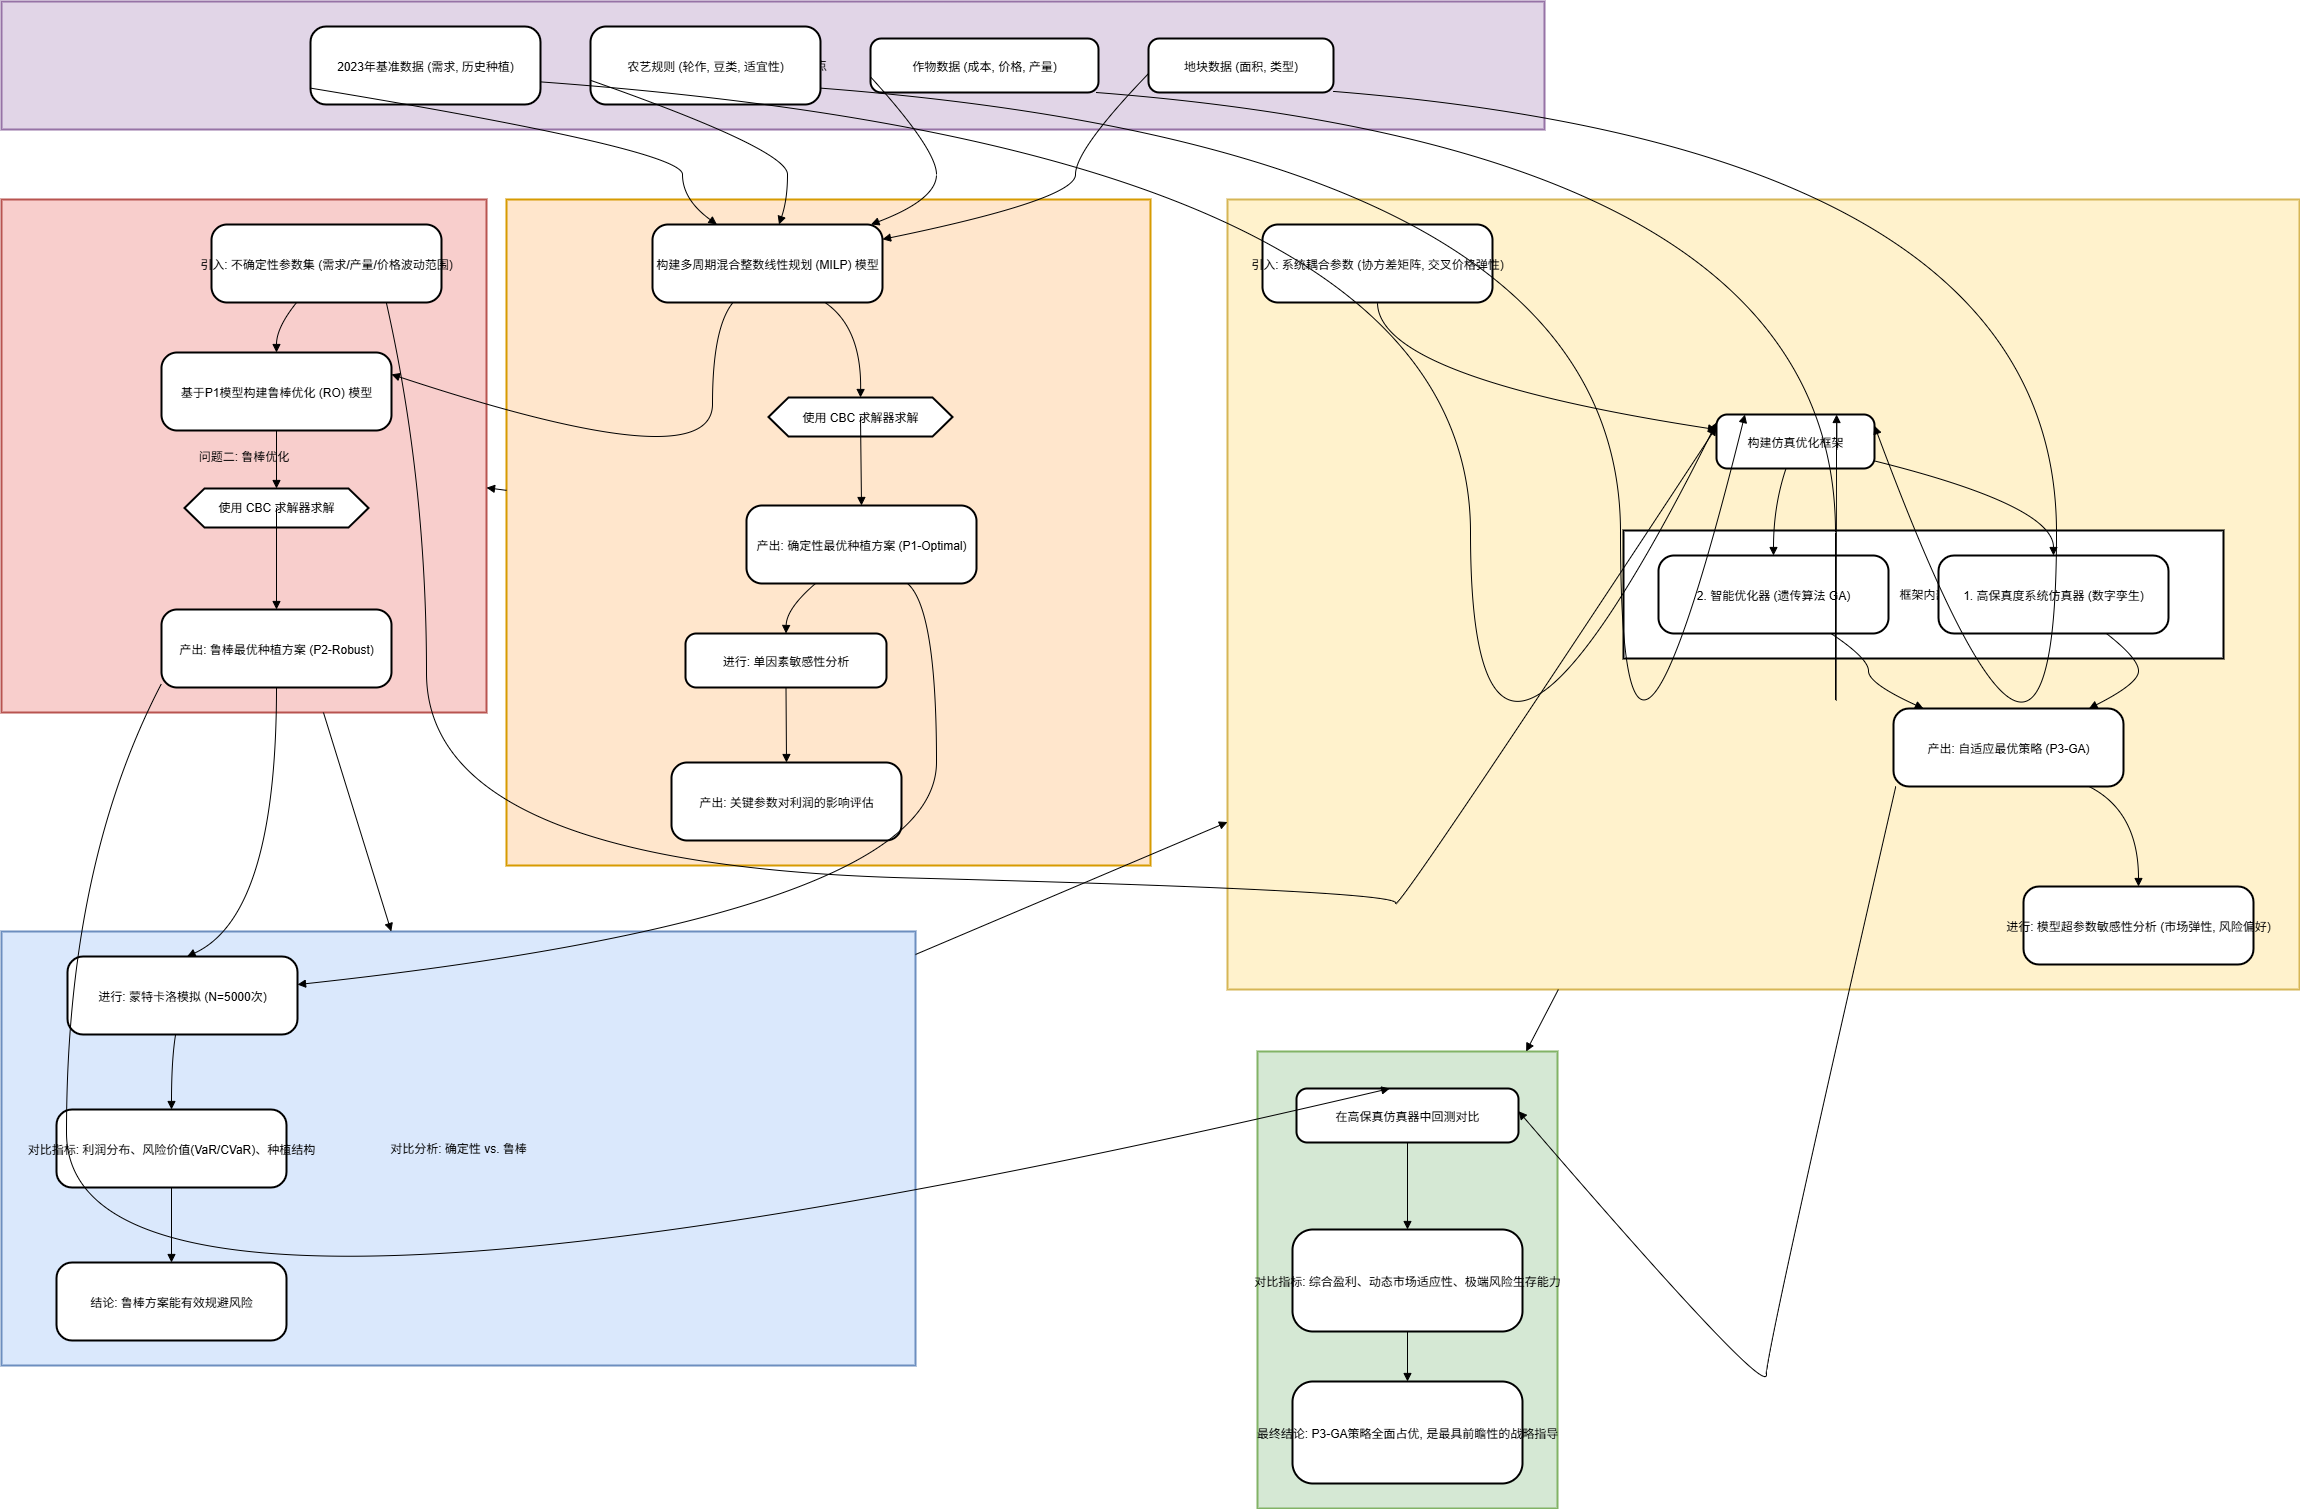
\includegraphics[width=0.7\textwidth]{../figures/all.png}
	\caption{整体框架}
	\label{fig:all}
\end{figure}


\section{模型假设}

\begin{enumerate}
	\item 假设2023年的农作物产量恰好满足当期市场需求,该年的产销数据可作为后续模型中市场预期销售量的基准。
	\item 假设附件所提供的全部数据均真实、准确,可作为模型的基础输入。
	\item 假设该乡村在农产品市场中为价格接受者,其任何一种作物的产量变化均不足以影响该作物的市场结算价格。
	\item 假设所有在预期内或可降价出售的农产品均能当季顺利售出,模型不考虑仓储、物流运输、市场交易以及产品损耗等环节产生的额外成本或收益影响。
\end{enumerate}


\section{符号说明}

\begin{table}[H]
	\centering
	\caption{符号说明}
	\begin{tabular}{ll}
		\toprule
		符号                 & 说明                                \\
		\midrule

		$i, I$             & 地块的索引与集合                          \\
		$j, J$             & 作物的索引与集合                          \\
		$k, K$             & 季节的索引与集合                          \\
		$y, Y$             & 年份的索引与集合(2024-2030)               \\
		$J_{\text{bean}}$  & 所有豆类作物的集合                         \\

		$A_i$              & 地块$i$ 的可用面积                       \\
		$C_j$              & 作物$j$ 的单位面积种植成本                   \\
		$P_j$              & 作物$j$ 的单位重量销售价格                   \\
		$\text{Yield}_j$   & 作物$j$ 的单位面积产量                     \\
		$\text{Demand}_j$  & 作物$j$ 的每季预期市场销售量                  \\
		$\text{Past}_{ij}$ & 地块$i$ 在2023年是否种植了作物 $j$ 的0-1参数    \\
		$S_{ijk}$          & 地块$i$ 在季节 $k$ 是否适宜种植作物 $j$ 的0-1参数 \\
		$A_{\min}$         & 单个地块上允许种植某种作物的最小面积阈值              \\
		$N_j$              & 作物$j$ 在单季内允许种植的最大分散地块数量           \\
		$M$                & 大M方法中的一个足够大的正数                    \\
		\bottomrule
	\end{tabular}
\end{table}